\pdfminorversion=4
\documentclass[]{article}
\usepackage[utf8]{inputenc}
\usepackage{amssymb,latexsym,amsmath}
\usepackage[a4paper,top=3cm,bottom=2cm,left=3cm,right=3cm,marginparwidth=1.75cm]{geometry}
\usepackage{graphicx}
\usepackage[colorlinks=true, allcolors=blue]{hyperref}
\begin{document}

    \begin{center}
    {\Large \textbf{\textsc{Langages formels - contrôle continu 1}}}
        \\
        ~\\
        {\Huge \textbf{\textsc{Sujet #NBSUJET#}}}\\
        ~\\
        Année \the\year
    \end{center}

    \vskip 5mm
    \textbf{Composer sur feuille papier; numérisez votre copie (photos, scanner), puis déposez-la sur Teams, dans l'équipe du cours de Langages Formels, dans le devoir "CC1" avant 13h50; prévoyez 10 minutes pour le scan/dépôt!} \\

    Essayez si possible de déposer un fichier PDF unique avec vos différentes pages, que vous pouvez obtenir avec une app du type CamScanner.


    \textbf{Les rendus en retard (après 13h50) pourront être pénalisés.}


    \emph{A composer seul. Les échanges avec toute autre personne sont interdits.}\\


    \section{(6 points)}
    \begin{figure}[htbp]
        \centering
        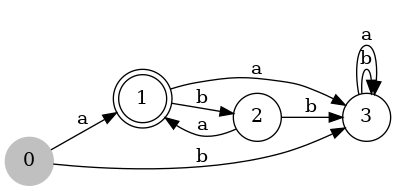
\includegraphics[width=15cm]{automateInitial.png}
        \caption{Initial}\label{fig:3.1}
    \end{figure}\

    \begin{enumerate}
        \item  Determiniser l'automate donné plus haut

        \item Minimiser l'automate donné plus haut

        \item Indiquer si les mots suivants sont reconnues par l'automate : {mots ..}

    \end{enumerate}

    %------------------

    \clearpage

    \begin{center}
    {\Large \textbf{\textsc}}
        \\
        ~\\
        {\Huge \textbf{\textsc{SOLUTIONS}}}\\
        ~\\
        Année \the\year
    \end{center}
    \begin{enumerate}
        \setcounter{enumi}{0}

        \begin{figure}[htbp]
            \centering
            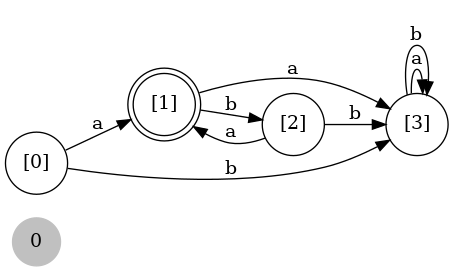
\includegraphics[width=15cm]{automateDeterministe.png}
            \caption{Deterministe.}\label{fig:3.1}
        \end{figure}\\
        \begin{figure}[htbp]
            \centering
            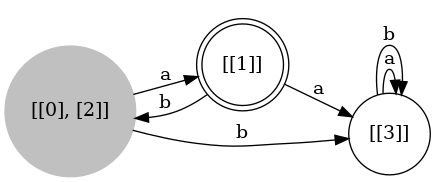
\includegraphics[width=15cm]{automateMinimal.png}
            \caption{Minimal}\label{fig:3.1}
        \end{figure}\\
        \begin{figure}[htbp]
            \centering
            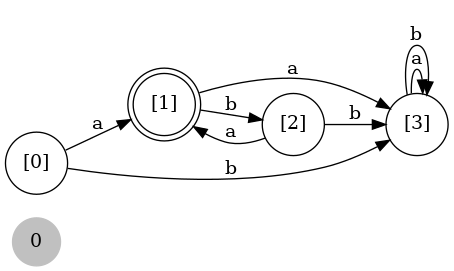
\includegraphics[width=15cm]{automateSynchro.png}
            \caption{Synchro}\label{fig:3.1}
        \end{figure}\\
    \end{enumerate}
    \setcounter{section}{0}
    \newpage


    \begin{center}
    {\Large \textbf{\textsc{Langages formels - contrôle continu 1}}}
        \\
        ~\\
        {\Huge \textbf{\textsc{Sujet #NBSUJET#}}}\\
        ~\\
        Année \the\year
    \end{center}

    \vskip 5mm
    \textbf{Composer sur feuille papier; numérisez votre copie (photos, scanner), puis déposez-la sur Teams, dans l'équipe du cours de Langages Formels, dans le devoir "CC1" avant 13h50; prévoyez 10 minutes pour le scan/dépôt!} \\

    Essayez si possible de déposer un fichier PDF unique avec vos différentes pages, que vous pouvez obtenir avec une app du type CamScanner.


    \textbf{Les rendus en retard (après 13h50) pourront être pénalisés.}


    \emph{A composer seul. Les échanges avec toute autre personne sont interdits.}\\


    \section{(6 points)}
    \begin{figure}[htbp]
        \centering
        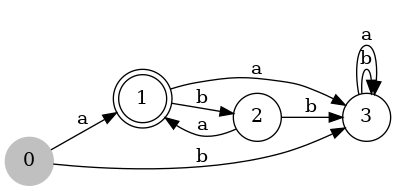
\includegraphics[width=15cm]{automateInitial.png}
        \caption{Initial}\label{fig:3.1}
    \end{figure}\

    \begin{enumerate}
        \item  Determiniser l'automate donné plus haut

        \item Minimiser l'automate donné plus haut

        \item Indiquer si les mots suivants sont reconnues par l'automate : {mots ..}

    \end{enumerate}

    %------------------

    \clearpage

    \begin{center}
    {\Large \textbf{\textsc}}
        \\
        ~\\
        {\Huge \textbf{\textsc{SOLUTIONS}}}\\
        ~\\
        Année \the\year
    \end{center}
    \begin{enumerate}
        \setcounter{enumi}{0}

        \begin{figure}[htbp]
            \centering
            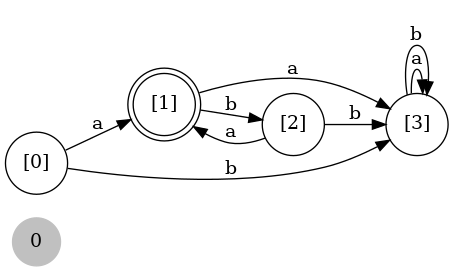
\includegraphics[width=15cm]{automateDeterministe.png}
            \caption{Deterministe.}\label{fig:3.1}
        \end{figure}\\
        \begin{figure}[htbp]
            \centering
            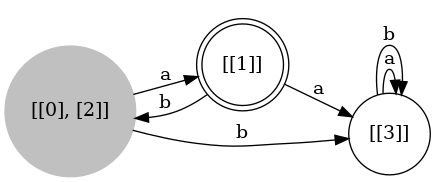
\includegraphics[width=15cm]{automateMinimal.png}
            \caption{Minimal}\label{fig:3.1}
        \end{figure}\\
        \begin{figure}[htbp]
            \centering
            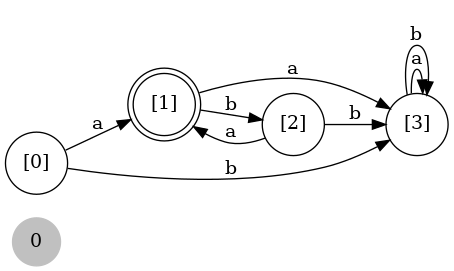
\includegraphics[width=15cm]{automateSynchro.png}
            \caption{Synchro}\label{fig:3.1}
        \end{figure}\\
    \end{enumerate}
    \setcounter{section}{0}
    \newpage
    \begin{center}
    {\Large \textbf{\textsc{Langages formels - contrôle continu 1}}}
        \\
        ~\\
        {\Huge \textbf{\textsc{Sujet #NBSUJET#}}}\\
        ~\\
        Année \the\year
    \end{center}

    \vskip 5mm
    \textbf{Composer sur feuille papier; numérisez votre copie (photos, scanner), puis déposez-la sur Teams, dans l'équipe du cours de Langages Formels, dans le devoir "CC1" avant 13h50; prévoyez 10 minutes pour le scan/dépôt!} \\

    Essayez si possible de déposer un fichier PDF unique avec vos différentes pages, que vous pouvez obtenir avec une app du type CamScanner.


    \textbf{Les rendus en retard (après 13h50) pourront être pénalisés.}


    \emph{A composer seul. Les échanges avec toute autre personne sont interdits.}\\


    \section{(6 points)}
    \begin{figure}[htbp]
        \centering
        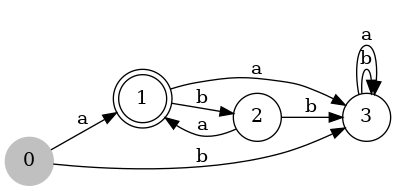
\includegraphics[width=15cm]{automateInitial.png}
        \caption{Initial}\label{fig:3.1}
    \end{figure}\

    \begin{enumerate}
        \item  Determiniser l'automate donné plus haut

        \item Minimiser l'automate donné plus haut

        \item Indiquer si les mots suivants sont reconnues par l'automate : {mots ..}

    \end{enumerate}

    %------------------

    \clearpage

    \begin{center}
    {\Large \textbf{\textsc}}
        \\
        ~\\
        {\Huge \textbf{\textsc{SOLUTIONS}}}\\
        ~\\
        Année \the\year
    \end{center}
    \begin{enumerate}
        \setcounter{enumi}{0}

        \begin{figure}[htbp]
            \centering
            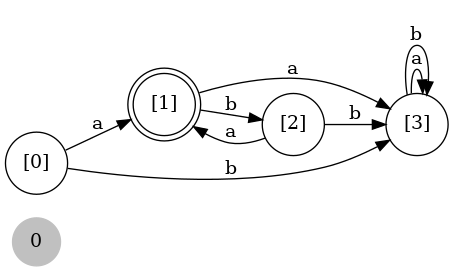
\includegraphics[width=15cm]{automateDeterministe.png}
            \caption{Deterministe.}\label{fig:3.1}
        \end{figure}\\
        \begin{figure}[htbp]
            \centering
            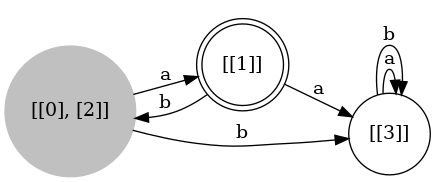
\includegraphics[width=15cm]{automateMinimal.png}
            \caption{Minimal}\label{fig:3.1}
        \end{figure}\\
        \begin{figure}[htbp]
            \centering
            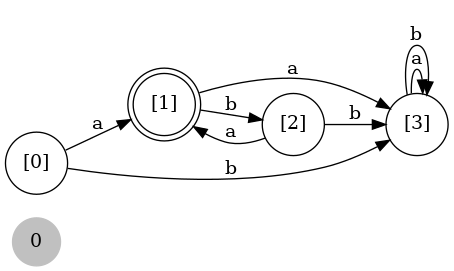
\includegraphics[width=15cm]{automateSynchro.png}
            \caption{Synchro}\label{fig:3.1}
        \end{figure}\\
    \end{enumerate}
    \setcounter{section}{0}
    \newpage
    \begin{center}
    {\Large \textbf{\textsc{Langages formels - contrôle continu 1}}}
        \\
        ~\\
        {\Huge \textbf{\textsc{Sujet #NBSUJET#}}}\\
        ~\\
        Année \the\year
    \end{center}

    \vskip 5mm
    \textbf{Composer sur feuille papier; numérisez votre copie (photos, scanner), puis déposez-la sur Teams, dans l'équipe du cours de Langages Formels, dans le devoir "CC1" avant 13h50; prévoyez 10 minutes pour le scan/dépôt!} \\

    Essayez si possible de déposer un fichier PDF unique avec vos différentes pages, que vous pouvez obtenir avec une app du type CamScanner.


    \textbf{Les rendus en retard (après 13h50) pourront être pénalisés.}


    \emph{A composer seul. Les échanges avec toute autre personne sont interdits.}\\


    \section{(6 points)}
    \begin{figure}[htbp]
        \centering
        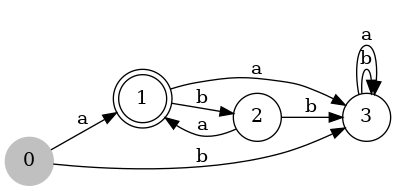
\includegraphics[width=15cm]{automateInitial.png}
        \caption{Initial}\label{fig:3.1}
    \end{figure}\

    \begin{enumerate}
        \item  Determiniser l'automate donné plus haut

        \item Minimiser l'automate donné plus haut

        \item Indiquer si les mots suivants sont reconnues par l'automate : {mots ..}

    \end{enumerate}

    %------------------

    \clearpage

    \begin{center}
    {\Large \textbf{\textsc}}
        \\
        ~\\
        {\Huge \textbf{\textsc{SOLUTIONS}}}\\
        ~\\
        Année \the\year
    \end{center}
    \begin{enumerate}
        \setcounter{enumi}{0}

        \begin{figure}[htbp]
            \centering
            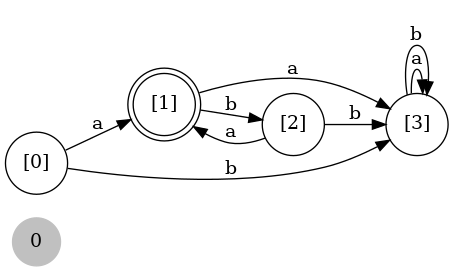
\includegraphics[width=15cm]{automateDeterministe.png}
            \caption{Deterministe.}\label{fig:3.1}
        \end{figure}\\
        \begin{figure}[htbp]
            \centering
            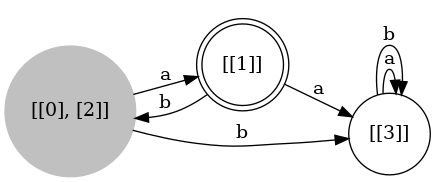
\includegraphics[width=15cm]{automateMinimal.png}
            \caption{Minimal}\label{fig:3.1}
        \end{figure}\\
        \begin{figure}[htbp]
            \centering
            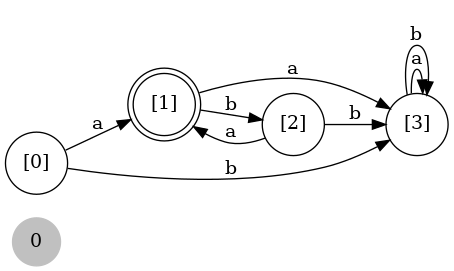
\includegraphics[width=15cm]{automateSynchro.png}
            \caption{Synchro}\label{fig:3.1}
        \end{figure}\\
    \end{enumerate}
    \setcounter{section}{0}
    \newpage
\end{document}
    \begin{center}
    {\Large \textbf{\textsc{Langages formels - contrôle continu 1}}}
        \\
        ~\\
        {\Huge \textbf{\textsc{Sujet #0#}}}\\
        ~\\
        Année \the\year
    \end{center}

    \vskip 5mm
    \textbf{Composer sur feuille papier; numérisez votre copie (photos, scanner), puis déposez-la sur Teams, dans l'équipe du cours de Langages Formels, dans le devoir "CC1" avant 13h50; prévoyez 10 minutes pour le scan/dépôt!} \\

    Essayez si possible de déposer un fichier PDF unique avec vos différentes pages, que vous pouvez obtenir avec une app du type CamScanner.


    \textbf{Les rendus en retard (après 13h50) pourront être pénalisés.}


    \emph{A composer seul. Les échanges avec toute autre personne sont interdits.}\\


    \section{(6 points)}
    \begin{figure}[htbp]
        \centering
        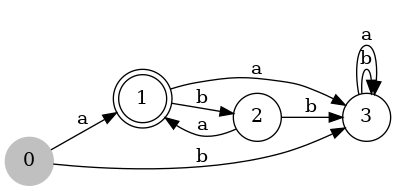
\includegraphics[width=15cm]{automateInitial.png}
        \caption{Initial}\label{fig:3.1}
    \end{figure}\

    \begin{enumerate}
        \item  Determiniser l'automate donné plus haut

        \item Minimiser l'automate donné plus haut

        \item Indiquer si les mots suivants sont reconnues par l'automate : {mots ..}

    \end{enumerate}

    %------------------

    \clearpage

    \begin{center}
    {\Large \textbf{\textsc}}
        \\
        ~\\
        {\Huge \textbf{\textsc{SOLUTIONS}}}\\
        ~\\
        Année \the\year
    \end{center}
    \begin{enumerate}
        \setcounter{enumi}{0}

        \begin{figure}[htbp]
            \centering
            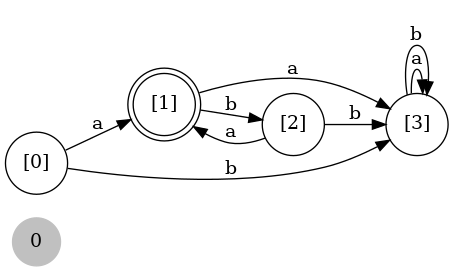
\includegraphics[width=15cm]{automateDeterministe.png}
            \caption{Deterministe.}\label{fig:3.1}
        \end{figure}\\
        \begin{figure}[htbp]
            \centering
            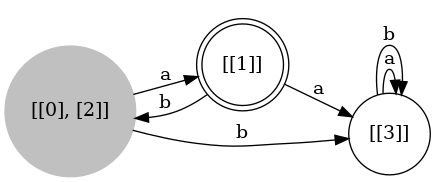
\includegraphics[width=15cm]{automateMinimal.png}
            \caption{Minimal}\label{fig:3.1}
        \end{figure}\\
        \begin{figure}[htbp]
            \centering
            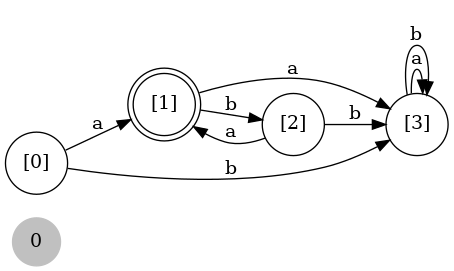
\includegraphics[width=15cm]{automateSynchro.png}
            \caption{Synchro}\label{fig:3.1}
        \end{figure}\\
    \end{enumerate}
    \setcounter{section}{0}
    \newpage
    \begin{center}
    {\Large \textbf{\textsc{Langages formels - contrôle continu 1}}}
        \\
        ~\\
        {\Huge \textbf{\textsc{Sujet #0#}}}\\
        ~\\
        Année \the\year
    \end{center}

    \vskip 5mm
    \textbf{Composer sur feuille papier; numérisez votre copie (photos, scanner), puis déposez-la sur Teams, dans l'équipe du cours de Langages Formels, dans le devoir "CC1" avant 13h50; prévoyez 10 minutes pour le scan/dépôt!} \\

    Essayez si possible de déposer un fichier PDF unique avec vos différentes pages, que vous pouvez obtenir avec une app du type CamScanner.


    \textbf{Les rendus en retard (après 13h50) pourront être pénalisés.}


    \emph{A composer seul. Les échanges avec toute autre personne sont interdits.}\\


    \section{(6 points)}
    \begin{figure}[htbp]
        \centering
        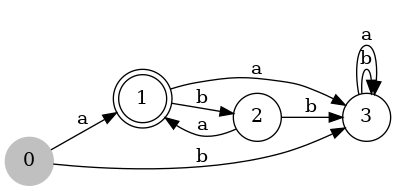
\includegraphics[width=15cm]{automateInitial.png}
        \caption{Initial}\label{fig:3.1}
    \end{figure}\

    \begin{enumerate}
        \item  Determiniser l'automate donné plus haut

        \item Minimiser l'automate donné plus haut

        \item Indiquer si les mots suivants sont reconnues par l'automate : {mots ..}

    \end{enumerate}

    %------------------

    \clearpage

    \begin{center}
    {\Large \textbf{\textsc}}
        \\
        ~\\
        {\Huge \textbf{\textsc{SOLUTIONS}}}\\
        ~\\
        Année \the\year
    \end{center}
    \begin{enumerate}
        \setcounter{enumi}{0}

        \begin{figure}[htbp]
            \centering
            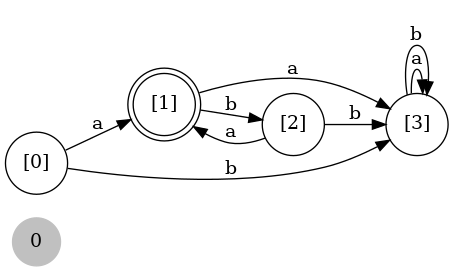
\includegraphics[width=15cm]{automateDeterministe.png}
            \caption{Deterministe.}\label{fig:3.1}
        \end{figure}\\
        \begin{figure}[htbp]
            \centering
            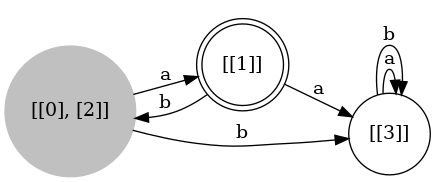
\includegraphics[width=15cm]{automateMinimal.png}
            \caption{Minimal}\label{fig:3.1}
        \end{figure}\\
        \begin{figure}[htbp]
            \centering
            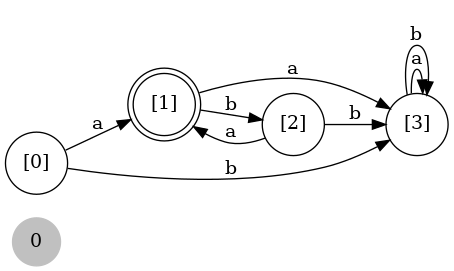
\includegraphics[width=15cm]{automateSynchro.png}
            \caption{Synchro}\label{fig:3.1}
        \end{figure}\\
    \end{enumerate}
    \setcounter{section}{0}
    \newpage
    \begin{center}
    {\Large \textbf{\textsc{Langages formels - contrôle continu 1}}}
        \\
        ~\\
        {\Huge \textbf{\textsc{Sujet #0#}}}\\
        ~\\
        Année \the\year
    \end{center}

    \vskip 5mm
    \textbf{Composer sur feuille papier; numérisez votre copie (photos, scanner), puis déposez-la sur Teams, dans l'équipe du cours de Langages Formels, dans le devoir "CC1" avant 13h50; prévoyez 10 minutes pour le scan/dépôt!} \\

    Essayez si possible de déposer un fichier PDF unique avec vos différentes pages, que vous pouvez obtenir avec une app du type CamScanner.


    \textbf{Les rendus en retard (après 13h50) pourront être pénalisés.}


    \emph{A composer seul. Les échanges avec toute autre personne sont interdits.}\\


    \section{(6 points)}
    \begin{figure}[htbp]
        \centering
        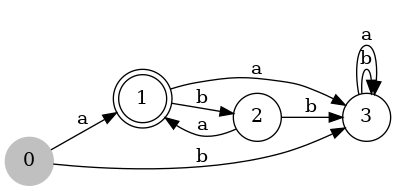
\includegraphics[width=15cm]{automateInitial.png}
        \caption{Initial}\label{fig:3.1}
    \end{figure}\

    \begin{enumerate}
        \item  Determiniser l'automate donné plus haut

        \item Minimiser l'automate donné plus haut

        \item Indiquer si les mots suivants sont reconnues par l'automate : {mots ..}

    \end{enumerate}

    %------------------

    \clearpage

    \begin{center}
    {\Large \textbf{\textsc}}
        \\
        ~\\
        {\Huge \textbf{\textsc{SOLUTIONS}}}\\
        ~\\
        Année \the\year
    \end{center}
    \begin{enumerate}
        \setcounter{enumi}{0}

        \begin{figure}[htbp]
            \centering
            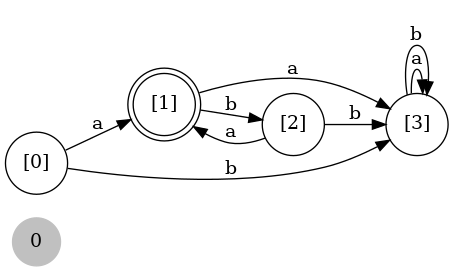
\includegraphics[width=15cm]{automateDeterministe.png}
            \caption{Deterministe.}\label{fig:3.1}
        \end{figure}\\
        \begin{figure}[htbp]
            \centering
            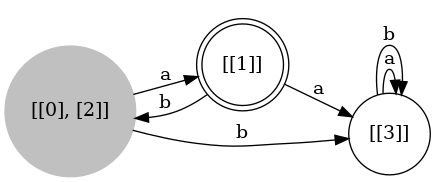
\includegraphics[width=15cm]{automateMinimal.png}
            \caption{Minimal}\label{fig:3.1}
        \end{figure}\\
        \begin{figure}[htbp]
            \centering
            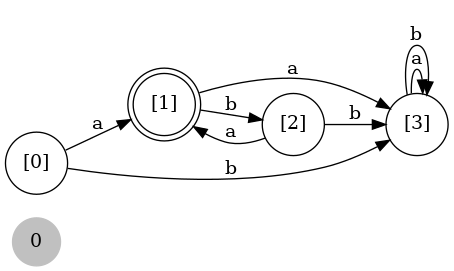
\includegraphics[width=15cm]{automateSynchro.png}
            \caption{Synchro}\label{fig:3.1}
        \end{figure}\\
    \end{enumerate}
    \setcounter{section}{0}
    \newpage
\end{document}
    \begin{center}
    {\Large \textbf{\textsc{Langages formels - contrôle continu 1}}}
        \\
        ~\\
        {\Huge \textbf{\textsc{Sujet #0 #}}}\\
        ~\\
        Année \the\year
    \end{center}

    \vskip 5mm
    \textbf{Composer sur feuille papier; numérisez votre copie (photos, scanner), puis déposez-la sur Teams, dans l'équipe du cours de Langages Formels, dans le devoir "CC1" avant 13h50; prévoyez 10 minutes pour le scan/dépôt!} \\

    Essayez si possible de déposer un fichier PDF unique avec vos différentes pages, que vous pouvez obtenir avec une app du type CamScanner.


    \textbf{Les rendus en retard (après 13h50) pourront être pénalisés.}


    \emph{A composer seul. Les échanges avec toute autre personne sont interdits.}\\


    \section{(6 points)}
    \begin{figure}[htbp]
        \centering
        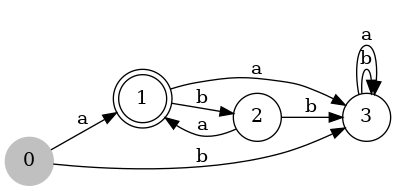
\includegraphics[width=15cm]{automateInitial.png}
        \caption{Initial}\label{fig:3.1}
    \end{figure}\

    \begin{enumerate}
        \item  Determiniser l'automate donné plus haut

        \item Minimiser l'automate donné plus haut

        \item Indiquer si les mots suivants sont reconnues par l'automate : {mots ..}

    \end{enumerate}

    %------------------

    \clearpage

    \begin{center}
    {\Large \textbf{\textsc}}
        \\
        ~\\
        {\Huge \textbf{\textsc{SOLUTIONS}}}\\
        ~\\
        Année \the\year
    \end{center}
    \begin{enumerate}
        \setcounter{enumi}{0}

        \begin{figure}[htbp]
            \centering
            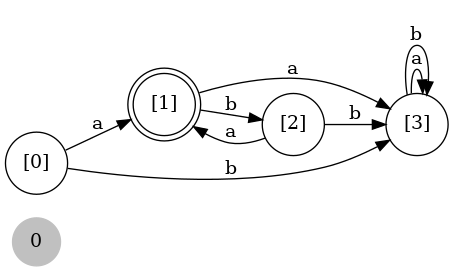
\includegraphics[width=15cm]{automateDeterministe.png}
            \caption{Deterministe.}\label{fig:3.1}
        \end{figure}\\
        \begin{figure}[htbp]
            \centering
            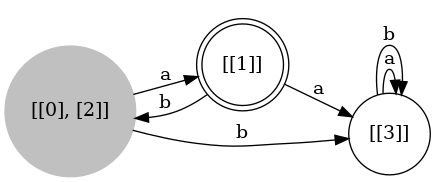
\includegraphics[width=15cm]{automateMinimal.png}
            \caption{Minimal}\label{fig:3.1}
        \end{figure}\\
        \begin{figure}[htbp]
            \centering
            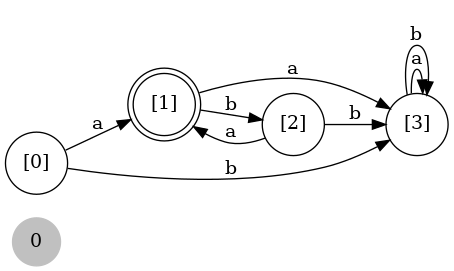
\includegraphics[width=15cm]{automateSynchro.png}
            \caption{Synchro}\label{fig:3.1}
        \end{figure}\\
    \end{enumerate}
    \setcounter{section}{0}
    \newpage
    \begin{center}
    {\Large \textbf{\textsc{Langages formels - contrôle continu 1}}}
        \\
        ~\\
        {\Huge \textbf{\textsc{Sujet #0 #}}}\\
        ~\\
        Année \the\year
    \end{center}

    \vskip 5mm
    \textbf{Composer sur feuille papier; numérisez votre copie (photos, scanner), puis déposez-la sur Teams, dans l'équipe du cours de Langages Formels, dans le devoir "CC1" avant 13h50; prévoyez 10 minutes pour le scan/dépôt!} \\

    Essayez si possible de déposer un fichier PDF unique avec vos différentes pages, que vous pouvez obtenir avec une app du type CamScanner.


    \textbf{Les rendus en retard (après 13h50) pourront être pénalisés.}


    \emph{A composer seul. Les échanges avec toute autre personne sont interdits.}\\


    \section{(6 points)}
    \begin{figure}[htbp]
        \centering
        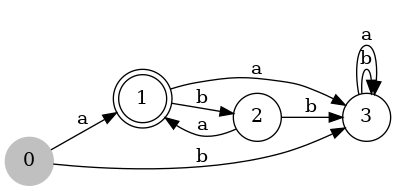
\includegraphics[width=15cm]{automateInitial.png}
        \caption{Initial}\label{fig:3.1}
    \end{figure}\

    \begin{enumerate}
        \item  Determiniser l'automate donné plus haut

        \item Minimiser l'automate donné plus haut

        \item Indiquer si les mots suivants sont reconnues par l'automate : {mots ..}

    \end{enumerate}

    %------------------

    \clearpage

    \begin{center}
    {\Large \textbf{\textsc}}
        \\
        ~\\
        {\Huge \textbf{\textsc{SOLUTIONS}}}\\
        ~\\
        Année \the\year
    \end{center}
    \begin{enumerate}
        \setcounter{enumi}{0}

        \begin{figure}[htbp]
            \centering
            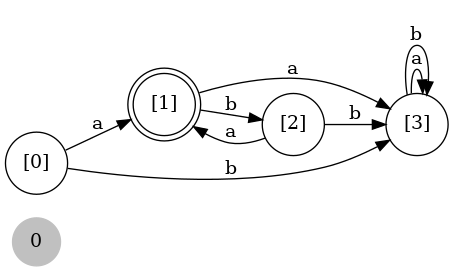
\includegraphics[width=15cm]{automateDeterministe.png}
            \caption{Deterministe.}\label{fig:3.1}
        \end{figure}\\
        \begin{figure}[htbp]
            \centering
            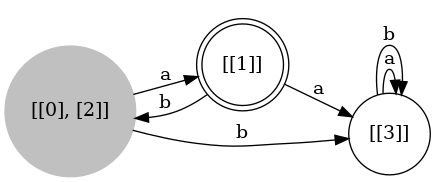
\includegraphics[width=15cm]{automateMinimal.png}
            \caption{Minimal}\label{fig:3.1}
        \end{figure}\\
        \begin{figure}[htbp]
            \centering
            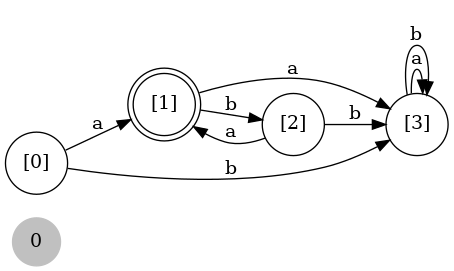
\includegraphics[width=15cm]{automateSynchro.png}
            \caption{Synchro}\label{fig:3.1}
        \end{figure}\\
    \end{enumerate}
    \setcounter{section}{0}
    \newpage
    \begin{center}
    {\Large \textbf{\textsc{Langages formels - contrôle continu 1}}}
        \\
        ~\\
        {\Huge \textbf{\textsc{Sujet #0 #}}}\\
        ~\\
        Année \the\year
    \end{center}

    \vskip 5mm
    \textbf{Composer sur feuille papier; numérisez votre copie (photos, scanner), puis déposez-la sur Teams, dans l'équipe du cours de Langages Formels, dans le devoir "CC1" avant 13h50; prévoyez 10 minutes pour le scan/dépôt!} \\

    Essayez si possible de déposer un fichier PDF unique avec vos différentes pages, que vous pouvez obtenir avec une app du type CamScanner.


    \textbf{Les rendus en retard (après 13h50) pourront être pénalisés.}


    \emph{A composer seul. Les échanges avec toute autre personne sont interdits.}\\


    \section{(6 points)}
    \begin{figure}[htbp]
        \centering
        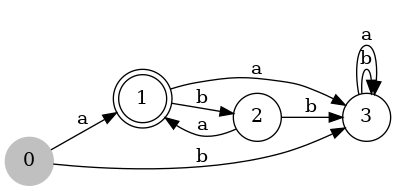
\includegraphics[width=15cm]{automateInitial.png}
        \caption{Initial}\label{fig:3.1}
    \end{figure}\

    \begin{enumerate}
        \item  Determiniser l'automate donné plus haut

        \item Minimiser l'automate donné plus haut

        \item Indiquer si les mots suivants sont reconnues par l'automate : {mots ..}

    \end{enumerate}

    %------------------

    \clearpage

    \begin{center}
    {\Large \textbf{\textsc}}
        \\
        ~\\
        {\Huge \textbf{\textsc{SOLUTIONS}}}\\
        ~\\
        Année \the\year
    \end{center}
    \begin{enumerate}
        \setcounter{enumi}{0}

        \begin{figure}[htbp]
            \centering
            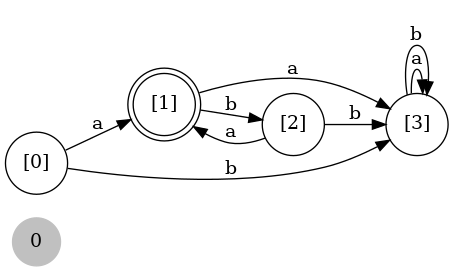
\includegraphics[width=15cm]{automateDeterministe.png}
            \caption{Deterministe.}\label{fig:3.1}
        \end{figure}\\
        \begin{figure}[htbp]
            \centering
            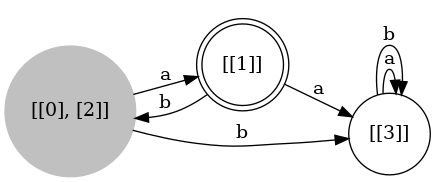
\includegraphics[width=15cm]{automateMinimal.png}
            \caption{Minimal}\label{fig:3.1}
        \end{figure}\\
        \begin{figure}[htbp]
            \centering
            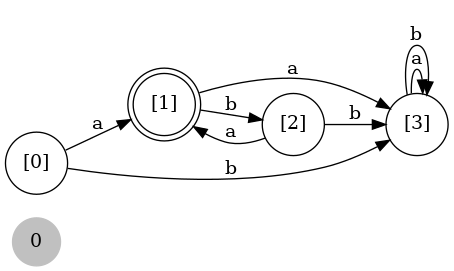
\includegraphics[width=15cm]{automateSynchro.png}
            \caption{Synchro}\label{fig:3.1}
        \end{figure}\\
    \end{enumerate}
    \setcounter{section}{0}
    \newpage
\end{document}
    \begin{center}
    {\Large \textbf{\textsc{Langages formels - contrôle continu 1}}}
        \\
        ~\\
        {\Huge \textbf{\textsc{Sujet 0 #}}}\\
        ~\\
        Année \the\year
    \end{center}

    \vskip 5mm
    \textbf{Composer sur feuille papier; numérisez votre copie (photos, scanner), puis déposez-la sur Teams, dans l'équipe du cours de Langages Formels, dans le devoir "CC1" avant 13h50; prévoyez 10 minutes pour le scan/dépôt!} \\

    Essayez si possible de déposer un fichier PDF unique avec vos différentes pages, que vous pouvez obtenir avec une app du type CamScanner.


    \textbf{Les rendus en retard (après 13h50) pourront être pénalisés.}


    \emph{A composer seul. Les échanges avec toute autre personne sont interdits.}\\


    \section{(6 points)}
    \begin{figure}[htbp]
        \centering
        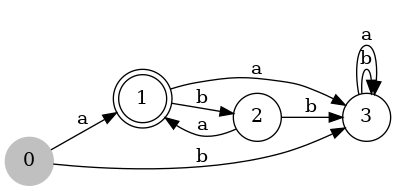
\includegraphics[width=15cm]{automateInitial.png}
        \caption{Initial}\label{fig:3.1}
    \end{figure}\

    \begin{enumerate}
        \item  Determiniser l'automate donné plus haut

        \item Minimiser l'automate donné plus haut

        \item Indiquer si les mots suivants sont reconnues par l'automate : {mots ..}

    \end{enumerate}

    %------------------

    \clearpage

    \begin{center}
    {\Large \textbf{\textsc}}
        \\
        ~\\
        {\Huge \textbf{\textsc{SOLUTIONS}}}\\
        ~\\
        Année \the\year
    \end{center}
    \begin{enumerate}
        \setcounter{enumi}{0}

        \begin{figure}[htbp]
            \centering
            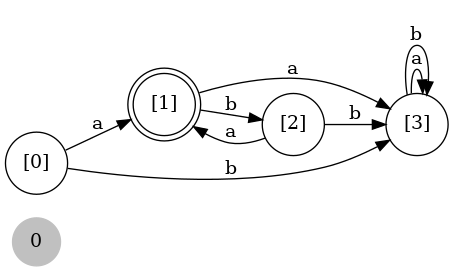
\includegraphics[width=15cm]{automateDeterministe.png}
            \caption{Deterministe.}\label{fig:3.1}
        \end{figure}\\
        \begin{figure}[htbp]
            \centering
            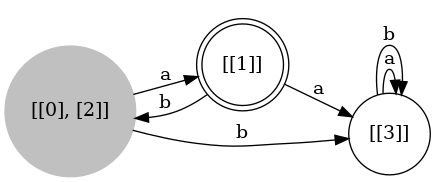
\includegraphics[width=15cm]{automateMinimal.png}
            \caption{Minimal}\label{fig:3.1}
        \end{figure}\\
        \begin{figure}[htbp]
            \centering
            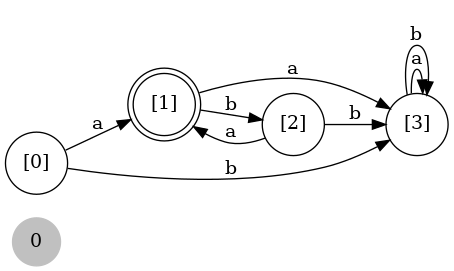
\includegraphics[width=15cm]{automateSynchro.png}
            \caption{Synchro}\label{fig:3.1}
        \end{figure}\\
    \end{enumerate}
    \setcounter{section}{0}
    \newpage
    \begin{center}
    {\Large \textbf{\textsc{Langages formels - contrôle continu 1}}}
        \\
        ~\\
        {\Huge \textbf{\textsc{Sujet 0 #}}}\\
        ~\\
        Année \the\year
    \end{center}

    \vskip 5mm
    \textbf{Composer sur feuille papier; numérisez votre copie (photos, scanner), puis déposez-la sur Teams, dans l'équipe du cours de Langages Formels, dans le devoir "CC1" avant 13h50; prévoyez 10 minutes pour le scan/dépôt!} \\

    Essayez si possible de déposer un fichier PDF unique avec vos différentes pages, que vous pouvez obtenir avec une app du type CamScanner.


    \textbf{Les rendus en retard (après 13h50) pourront être pénalisés.}


    \emph{A composer seul. Les échanges avec toute autre personne sont interdits.}\\


    \section{(6 points)}
    \begin{figure}[htbp]
        \centering
        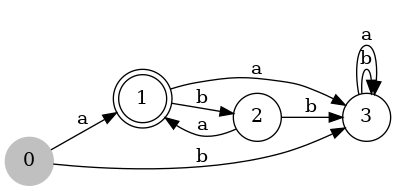
\includegraphics[width=15cm]{automateInitial.png}
        \caption{Initial}\label{fig:3.1}
    \end{figure}\

    \begin{enumerate}
        \item  Determiniser l'automate donné plus haut

        \item Minimiser l'automate donné plus haut

        \item Indiquer si les mots suivants sont reconnues par l'automate : {mots ..}

    \end{enumerate}

    %------------------

    \clearpage

    \begin{center}
    {\Large \textbf{\textsc}}
        \\
        ~\\
        {\Huge \textbf{\textsc{SOLUTIONS}}}\\
        ~\\
        Année \the\year
    \end{center}
    \begin{enumerate}
        \setcounter{enumi}{0}

        \begin{figure}[htbp]
            \centering
            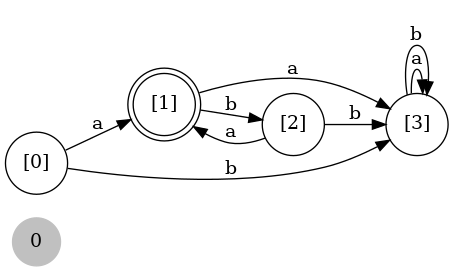
\includegraphics[width=15cm]{automateDeterministe.png}
            \caption{Deterministe.}\label{fig:3.1}
        \end{figure}\\
        \begin{figure}[htbp]
            \centering
            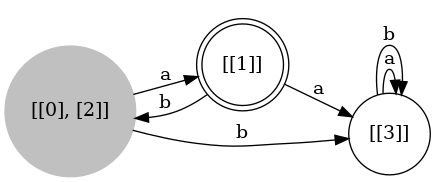
\includegraphics[width=15cm]{automateMinimal.png}
            \caption{Minimal}\label{fig:3.1}
        \end{figure}\\
        \begin{figure}[htbp]
            \centering
            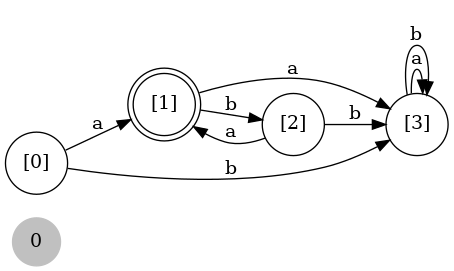
\includegraphics[width=15cm]{automateSynchro.png}
            \caption{Synchro}\label{fig:3.1}
        \end{figure}\\
    \end{enumerate}
    \setcounter{section}{0}
    \newpage
    \begin{center}
    {\Large \textbf{\textsc{Langages formels - contrôle continu 1}}}
        \\
        ~\\
        {\Huge \textbf{\textsc{Sujet 0 #}}}\\
        ~\\
        Année \the\year
    \end{center}

    \vskip 5mm
    \textbf{Composer sur feuille papier; numérisez votre copie (photos, scanner), puis déposez-la sur Teams, dans l'équipe du cours de Langages Formels, dans le devoir "CC1" avant 13h50; prévoyez 10 minutes pour le scan/dépôt!} \\

    Essayez si possible de déposer un fichier PDF unique avec vos différentes pages, que vous pouvez obtenir avec une app du type CamScanner.


    \textbf{Les rendus en retard (après 13h50) pourront être pénalisés.}


    \emph{A composer seul. Les échanges avec toute autre personne sont interdits.}\\


    \section{(6 points)}
    \begin{figure}[htbp]
        \centering
        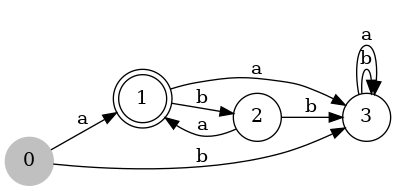
\includegraphics[width=15cm]{automateInitial.png}
        \caption{Initial}\label{fig:3.1}
    \end{figure}\

    \begin{enumerate}
        \item  Determiniser l'automate donné plus haut

        \item Minimiser l'automate donné plus haut

        \item Indiquer si les mots suivants sont reconnues par l'automate : {mots ..}

    \end{enumerate}

    %------------------

    \clearpage

    \begin{center}
    {\Large \textbf{\textsc}}
        \\
        ~\\
        {\Huge \textbf{\textsc{SOLUTIONS}}}\\
        ~\\
        Année \the\year
    \end{center}
    \begin{enumerate}
        \setcounter{enumi}{0}

        \begin{figure}[htbp]
            \centering
            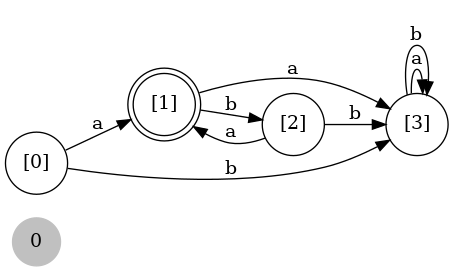
\includegraphics[width=15cm]{automateDeterministe.png}
            \caption{Deterministe.}\label{fig:3.1}
        \end{figure}\\
        \begin{figure}[htbp]
            \centering
            \includegraphics[width=15cm]{automateMinimal.png}
            \caption{Minimal}\label{fig:3.1}
        \end{figure}\\
        \begin{figure}[htbp]
            \centering
            \includegraphics[width=15cm]{automateSynchro.png}
            \caption{Synchro}\label{fig:3.1}
        \end{figure}\\
    \end{enumerate}
    \setcounter{section}{0}
    \newpage
\end{document}
    \begin{center}
    {\Large \textbf{\textsc{Langages formels - contrôle continu 1}}}
        \\
        ~\\
        {\Huge \textbf{\textsc{Sujet 0#}}}\\
        ~\\
        Année \the\year
    \end{center}

    \vskip 5mm
    \textbf{Composer sur feuille papier; numérisez votre copie (photos, scanner), puis déposez-la sur Teams, dans l'équipe du cours de Langages Formels, dans le devoir "CC1" avant 13h50; prévoyez 10 minutes pour le scan/dépôt!} \\

    Essayez si possible de déposer un fichier PDF unique avec vos différentes pages, que vous pouvez obtenir avec une app du type CamScanner.


    \textbf{Les rendus en retard (après 13h50) pourront être pénalisés.}


    \emph{A composer seul. Les échanges avec toute autre personne sont interdits.}\\


    \section{(6 points)}
    \begin{figure}[htbp]
        \centering
        \includegraphics[width=15cm]{automateInitial.png}
        \caption{Initial}\label{fig:3.1}
    \end{figure}\

    \begin{enumerate}
        \item  Determiniser l'automate donné plus haut

        \item Minimiser l'automate donné plus haut

        \item Indiquer si les mots suivants sont reconnues par l'automate : {mots ..}

    \end{enumerate}

    %------------------

    \clearpage

    \begin{center}
    {\Large \textbf{\textsc}}
        \\
        ~\\
        {\Huge \textbf{\textsc{SOLUTIONS}}}\\
        ~\\
        Année \the\year
    \end{center}
    \begin{enumerate}
        \setcounter{enumi}{0}

        \begin{figure}[htbp]
            \centering
            \includegraphics[width=15cm]{automateDeterministe.png}
            \caption{Deterministe.}\label{fig:3.1}
        \end{figure}\\
        \begin{figure}[htbp]
            \centering
            \includegraphics[width=15cm]{automateMinimal.png}
            \caption{Minimal}\label{fig:3.1}
        \end{figure}\\
        \begin{figure}[htbp]
            \centering
            \includegraphics[width=15cm]{automateSynchro.png}
            \caption{Synchro}\label{fig:3.1}
        \end{figure}\\
    \end{enumerate}
    \setcounter{section}{0}
    \newpage
    \begin{center}
    {\Large \textbf{\textsc{Langages formels - contrôle continu 1}}}
        \\
        ~\\
        {\Huge \textbf{\textsc{Sujet 0#}}}\\
        ~\\
        Année \the\year
    \end{center}

    \vskip 5mm
    \textbf{Composer sur feuille papier; numérisez votre copie (photos, scanner), puis déposez-la sur Teams, dans l'équipe du cours de Langages Formels, dans le devoir "CC1" avant 13h50; prévoyez 10 minutes pour le scan/dépôt!} \\

    Essayez si possible de déposer un fichier PDF unique avec vos différentes pages, que vous pouvez obtenir avec une app du type CamScanner.


    \textbf{Les rendus en retard (après 13h50) pourront être pénalisés.}


    \emph{A composer seul. Les échanges avec toute autre personne sont interdits.}\\


    \section{(6 points)}
    \begin{figure}[htbp]
        \centering
        \includegraphics[width=15cm]{automateInitial.png}
        \caption{Initial}\label{fig:3.1}
    \end{figure}\

    \begin{enumerate}
        \item  Determiniser l'automate donné plus haut

        \item Minimiser l'automate donné plus haut

        \item Indiquer si les mots suivants sont reconnues par l'automate : {mots ..}

    \end{enumerate}

    %------------------

    \clearpage

    \begin{center}
    {\Large \textbf{\textsc}}
        \\
        ~\\
        {\Huge \textbf{\textsc{SOLUTIONS}}}\\
        ~\\
        Année \the\year
    \end{center}
    \begin{enumerate}
        \setcounter{enumi}{0}

        \begin{figure}[htbp]
            \centering
            \includegraphics[width=15cm]{automateDeterministe.png}
            \caption{Deterministe.}\label{fig:3.1}
        \end{figure}\\
        \begin{figure}[htbp]
            \centering
            \includegraphics[width=15cm]{automateMinimal.png}
            \caption{Minimal}\label{fig:3.1}
        \end{figure}\\
        \begin{figure}[htbp]
            \centering
            \includegraphics[width=15cm]{automateSynchro.png}
            \caption{Synchro}\label{fig:3.1}
        \end{figure}\\
    \end{enumerate}
    \setcounter{section}{0}
    \newpage
    \begin{center}
    {\Large \textbf{\textsc{Langages formels - contrôle continu 1}}}
        \\
        ~\\
        {\Huge \textbf{\textsc{Sujet 0#}}}\\
        ~\\
        Année \the\year
    \end{center}

    \vskip 5mm
    \textbf{Composer sur feuille papier; numérisez votre copie (photos, scanner), puis déposez-la sur Teams, dans l'équipe du cours de Langages Formels, dans le devoir "CC1" avant 13h50; prévoyez 10 minutes pour le scan/dépôt!} \\

    Essayez si possible de déposer un fichier PDF unique avec vos différentes pages, que vous pouvez obtenir avec une app du type CamScanner.


    \textbf{Les rendus en retard (après 13h50) pourront être pénalisés.}


    \emph{A composer seul. Les échanges avec toute autre personne sont interdits.}\\


    \section{(6 points)}
    \begin{figure}[htbp]
        \centering
        \includegraphics[width=15cm]{automateInitial.png}
        \caption{Initial}\label{fig:3.1}
    \end{figure}\

    \begin{enumerate}
        \item  Determiniser l'automate donné plus haut

        \item Minimiser l'automate donné plus haut

        \item Indiquer si les mots suivants sont reconnues par l'automate : {mots ..}

    \end{enumerate}

    %------------------

    \clearpage

    \begin{center}
    {\Large \textbf{\textsc}}
        \\
        ~\\
        {\Huge \textbf{\textsc{SOLUTIONS}}}\\
        ~\\
        Année \the\year
    \end{center}
    \begin{enumerate}
        \setcounter{enumi}{0}

        \begin{figure}[htbp]
            \centering
            \includegraphics[width=15cm]{automateDeterministe.png}
            \caption{Deterministe.}\label{fig:3.1}
        \end{figure}\\
        \begin{figure}[htbp]
            \centering
            \includegraphics[width=15cm]{automateMinimal.png}
            \caption{Minimal}\label{fig:3.1}
        \end{figure}\\
        \begin{figure}[htbp]
            \centering
            \includegraphics[width=15cm]{automateSynchro.png}
            \caption{Synchro}\label{fig:3.1}
        \end{figure}\\
    \end{enumerate}
    \setcounter{section}{0}
    \newpage
\end{document}
    \begin{center}
    {\Large \textbf{\textsc{Langages formels - contrôle continu 1}}}
        \\
        ~\\
        {\Huge \textbf{\textsc{Sujet 0#}}}\\
        ~\\
        Année \the\year
    \end{center}

    \vskip 5mm
    \textbf{Composer sur feuille papier; numérisez votre copie (photos, scanner), puis déposez-la sur Teams, dans l'équipe du cours de Langages Formels, dans le devoir "CC1" avant 13h50; prévoyez 10 minutes pour le scan/dépôt!} \\

    Essayez si possible de déposer un fichier PDF unique avec vos différentes pages, que vous pouvez obtenir avec une app du type CamScanner.


    \textbf{Les rendus en retard (après 13h50) pourront être pénalisés.}


    \emph{A composer seul. Les échanges avec toute autre personne sont interdits.}\\


    \section{(6 points)}
    \begin{figure}[htbp]
        \centering
        \includegraphics[width=15cm]{automateInitial.png}
        \caption{Initial}\label{fig:3.1}
    \end{figure}\

    \begin{enumerate}
        \item  Determiniser l'automate donné plus haut

        \item Minimiser l'automate donné plus haut

        \item Indiquer si les mots suivants sont reconnues par l'automate : {mots ..}

    \end{enumerate}

    %------------------

    \newpage

    \begin{center}
    {\Large \textbf{\textsc}}
        \\
        ~\\
        {\Huge \textbf{\textsc{SOLUTIONS}}}\\
        ~\\
        Année \the\year
    \end{center}
    \begin{enumerate}
        \setcounter{enumi}{0}

        \begin{figure}[htbp]
            \centering
            \includegraphics[width=15cm]{automateDeterministe.png}
            \caption{Deterministe.}\label{fig:3.1}
        \end{figure}\\
        \begin{figure}[htbp]
            \centering
            \includegraphics[width=15cm]{automateMinimal.png}
            \caption{Minimal}\label{fig:3.1}
        \end{figure}\\
        \begin{figure}[htbp]
            \centering
            \includegraphics[width=15cm]{automateSynchro.png}
            \caption{Synchro}\label{fig:3.1}
        \end{figure}\\
    \end{enumerate}
    \setcounter{section}{0}
    \newpage
    \begin{center}
    {\Large \textbf{\textsc{Langages formels - contrôle continu 1}}}
        \\
        ~\\
        {\Huge \textbf{\textsc{Sujet 0#}}}\\
        ~\\
        Année \the\year
    \end{center}

    \vskip 5mm
    \textbf{Composer sur feuille papier; numérisez votre copie (photos, scanner), puis déposez-la sur Teams, dans l'équipe du cours de Langages Formels, dans le devoir "CC1" avant 13h50; prévoyez 10 minutes pour le scan/dépôt!} \\

    Essayez si possible de déposer un fichier PDF unique avec vos différentes pages, que vous pouvez obtenir avec une app du type CamScanner.


    \textbf{Les rendus en retard (après 13h50) pourront être pénalisés.}


    \emph{A composer seul. Les échanges avec toute autre personne sont interdits.}\\


    \section{(6 points)}
    \begin{figure}[htbp]
        \centering
        \includegraphics[width=15cm]{automateInitial.png}
        \caption{Initial}\label{fig:3.1}
    \end{figure}\

    \begin{enumerate}
        \item  Determiniser l'automate donné plus haut

        \item Minimiser l'automate donné plus haut

        \item Indiquer si les mots suivants sont reconnues par l'automate : {mots ..}

    \end{enumerate}

    %------------------

    \newpage

    \begin{center}
    {\Large \textbf{\textsc}}
        \\
        ~\\
        {\Huge \textbf{\textsc{SOLUTIONS}}}\\
        ~\\
        Année \the\year
    \end{center}
    \begin{enumerate}
        \setcounter{enumi}{0}

        \begin{figure}[htbp]
            \centering
            \includegraphics[width=15cm]{automateDeterministe.png}
            \caption{Deterministe.}\label{fig:3.1}
        \end{figure}\\
        \begin{figure}[htbp]
            \centering
            \includegraphics[width=15cm]{automateMinimal.png}
            \caption{Minimal}\label{fig:3.1}
        \end{figure}\\
        \begin{figure}[htbp]
            \centering
            \includegraphics[width=15cm]{automateSynchro.png}
            \caption{Synchro}\label{fig:3.1}
        \end{figure}\\
    \end{enumerate}
    \setcounter{section}{0}
    \newpage
    \begin{center}
    {\Large \textbf{\textsc{Langages formels - contrôle continu 1}}}
        \\
        ~\\
        {\Huge \textbf{\textsc{Sujet 0#}}}\\
        ~\\
        Année \the\year
    \end{center}

    \vskip 5mm
    \textbf{Composer sur feuille papier; numérisez votre copie (photos, scanner), puis déposez-la sur Teams, dans l'équipe du cours de Langages Formels, dans le devoir "CC1" avant 13h50; prévoyez 10 minutes pour le scan/dépôt!} \\

    Essayez si possible de déposer un fichier PDF unique avec vos différentes pages, que vous pouvez obtenir avec une app du type CamScanner.


    \textbf{Les rendus en retard (après 13h50) pourront être pénalisés.}


    \emph{A composer seul. Les échanges avec toute autre personne sont interdits.}\\


    \section{(6 points)}
    \begin{figure}[htbp]
        \centering
        \includegraphics[width=15cm]{automateInitial.png}
        \caption{Initial}\label{fig:3.1}
    \end{figure}\

    \begin{enumerate}
        \item  Determiniser l'automate donné plus haut

        \item Minimiser l'automate donné plus haut

        \item Indiquer si les mots suivants sont reconnues par l'automate : {mots ..}

    \end{enumerate}

    %------------------

    \newpage

    \begin{center}
    {\Large \textbf{\textsc}}
        \\
        ~\\
        {\Huge \textbf{\textsc{SOLUTIONS}}}\\
        ~\\
        Année \the\year
    \end{center}
    \begin{enumerate}
        \setcounter{enumi}{0}

        \begin{figure}[htbp]
            \centering
            \includegraphics[width=15cm]{automateDeterministe.png}
            \caption{Deterministe.}\label{fig:3.1}
        \end{figure}\\
        \begin{figure}[htbp]
            \centering
            \includegraphics[width=15cm]{automateMinimal.png}
            \caption{Minimal}\label{fig:3.1}
        \end{figure}\\
        \begin{figure}[htbp]
            \centering
            \includegraphics[width=15cm]{automateSynchro.png}
            \caption{Synchro}\label{fig:3.1}
        \end{figure}\\
    \end{enumerate}
    \setcounter{section}{0}
    \newpage
\end{document}
    \begin{center}
    {\Large \textbf{\textsc{Langages formels - contrôle continu 1}}}
        \\
        ~\\
        {\Huge \textbf{\textsc{Sujet 0}}}\\
        ~\\
        Année \the\year
    \end{center}

    \vskip 5mm
    \textbf{Composer sur feuille papier; numérisez votre copie (photos, scanner), puis déposez-la sur Teams, dans l'équipe du cours de Langages Formels, dans le devoir "CC1" avant 13h50; prévoyez 10 minutes pour le scan/dépôt!} \\

    Essayez si possible de déposer un fichier PDF unique avec vos différentes pages, que vous pouvez obtenir avec une app du type CamScanner.


    \textbf{Les rendus en retard (après 13h50) pourront être pénalisés.}


    \emph{A composer seul. Les échanges avec toute autre personne sont interdits.}\\


    \section{(6 points)}
    \begin{figure}[htbp]
        \centering
        \includegraphics[width=15cm]{automateInitial.png}
        \caption{Initial}\label{fig:3.1}
    \end{figure}\

    \begin{enumerate}
        \item  Determiniser l'automate donné plus haut

        \item Minimiser l'automate donné plus haut

        \item Indiquer si les mots suivants sont reconnues par l'automate : {mots ..}

    \end{enumerate}

    %------------------

    \newpage

    \begin{center}
    {\Large \textbf{\textsc}}
        \\
        ~\\
        {\Huge \textbf{\textsc{SOLUTIONS}}}\\
        ~\\
        Année \the\year
    \end{center}
    \begin{enumerate}
        \setcounter{enumi}{0}

        \begin{figure}[htbp]
            \centering
            \includegraphics[width=15cm]{automateDeterministe.png}
            \caption{Deterministe.}\label{fig:3.1}
        \end{figure}\\
        \begin{figure}[htbp]
            \centering
            \includegraphics[width=15cm]{automateMinimal.png}
            \caption{Minimal}\label{fig:3.1}
        \end{figure}\\
        \begin{figure}[htbp]
            \centering
            \includegraphics[width=15cm]{automateSynchro.png}
            \caption{Synchro}\label{fig:3.1}
        \end{figure}\\
    \end{enumerate}
    \setcounter{section}{0}
    \newpage
    \begin{center}
    {\Large \textbf{\textsc{Langages formels - contrôle continu 1}}}
        \\
        ~\\
        {\Huge \textbf{\textsc{Sujet 0}}}\\
        ~\\
        Année \the\year
    \end{center}

    \vskip 5mm
    \textbf{Composer sur feuille papier; numérisez votre copie (photos, scanner), puis déposez-la sur Teams, dans l'équipe du cours de Langages Formels, dans le devoir "CC1" avant 13h50; prévoyez 10 minutes pour le scan/dépôt!} \\

    Essayez si possible de déposer un fichier PDF unique avec vos différentes pages, que vous pouvez obtenir avec une app du type CamScanner.


    \textbf{Les rendus en retard (après 13h50) pourront être pénalisés.}


    \emph{A composer seul. Les échanges avec toute autre personne sont interdits.}\\


    \section{(6 points)}
    \begin{figure}[htbp]
        \centering
        \includegraphics[width=15cm]{automateInitial.png}
        \caption{Initial}\label{fig:3.1}
    \end{figure}\

    \begin{enumerate}
        \item  Determiniser l'automate donné plus haut

        \item Minimiser l'automate donné plus haut

        \item Indiquer si les mots suivants sont reconnues par l'automate : {mots ..}

    \end{enumerate}

    %------------------

    \newpage

    \begin{center}
    {\Large \textbf{\textsc}}
        \\
        ~\\
        {\Huge \textbf{\textsc{SOLUTIONS}}}\\
        ~\\
        Année \the\year
    \end{center}
    \begin{enumerate}
        \setcounter{enumi}{0}

        \begin{figure}[htbp]
            \centering
            \includegraphics[width=15cm]{automateDeterministe.png}
            \caption{Deterministe.}\label{fig:3.1}
        \end{figure}\\
        \begin{figure}[htbp]
            \centering
            \includegraphics[width=15cm]{automateMinimal.png}
            \caption{Minimal}\label{fig:3.1}
        \end{figure}\\
        \begin{figure}[htbp]
            \centering
            \includegraphics[width=15cm]{automateSynchro.png}
            \caption{Synchro}\label{fig:3.1}
        \end{figure}\\
    \end{enumerate}
    \setcounter{section}{0}
    \newpage
    \begin{center}
    {\Large \textbf{\textsc{Langages formels - contrôle continu 1}}}
        \\
        ~\\
        {\Huge \textbf{\textsc{Sujet 0}}}\\
        ~\\
        Année \the\year
    \end{center}

    \vskip 5mm
    \textbf{Composer sur feuille papier; numérisez votre copie (photos, scanner), puis déposez-la sur Teams, dans l'équipe du cours de Langages Formels, dans le devoir "CC1" avant 13h50; prévoyez 10 minutes pour le scan/dépôt!} \\

    Essayez si possible de déposer un fichier PDF unique avec vos différentes pages, que vous pouvez obtenir avec une app du type CamScanner.


    \textbf{Les rendus en retard (après 13h50) pourront être pénalisés.}


    \emph{A composer seul. Les échanges avec toute autre personne sont interdits.}\\


    \section{(6 points)}
    \begin{figure}[htbp]
        \centering
        \includegraphics[width=15cm]{automateInitial.png}
        \caption{Initial}\label{fig:3.1}
    \end{figure}\

    \begin{enumerate}
        \item  Determiniser l'automate donné plus haut

        \item Minimiser l'automate donné plus haut

        \item Indiquer si les mots suivants sont reconnues par l'automate : {mots ..}

    \end{enumerate}

    %------------------

    \newpage

    \begin{center}
    {\Large \textbf{\textsc}}
        \\
        ~\\
        {\Huge \textbf{\textsc{SOLUTIONS}}}\\
        ~\\
        Année \the\year
    \end{center}
    \begin{enumerate}
        \setcounter{enumi}{0}

        \begin{figure}[htbp]
            \centering
            \includegraphics[width=15cm]{automateDeterministe.png}
            \caption{Deterministe.}\label{fig:3.1}
        \end{figure}\\
        \begin{figure}[htbp]
            \centering
            \includegraphics[width=15cm]{automateMinimal.png}
            \caption{Minimal}\label{fig:3.1}
        \end{figure}\\
        \begin{figure}[htbp]
            \centering
            \includegraphics[width=15cm]{automateSynchro.png}
            \caption{Synchro}\label{fig:3.1}
        \end{figure}\\
    \end{enumerate}
    \setcounter{section}{0}
    \newpage
\end{document}
    \begin{center}
    {\Large \textbf{\textsc{Langages formels - contrôle continu 1}}}
        \\
        ~\\
        {\Huge \textbf{\textsc{Sujet 0}}}\\
        ~\\
        Année \the\year
    \end{center}

    \vskip 5mm
    \textbf{Composer sur feuille papier; numérisez votre copie (photos, scanner), puis déposez-la sur Teams, dans l'équipe du cours de Langages Formels, dans le devoir "CC1" avant 13h50; prévoyez 10 minutes pour le scan/dépôt!} \\

    Essayez si possible de déposer un fichier PDF unique avec vos différentes pages, que vous pouvez obtenir avec une app du type CamScanner.


    \textbf{Les rendus en retard (après 13h50) pourront être pénalisés.}


    \emph{A composer seul. Les échanges avec toute autre personne sont interdits.}\\


    \section{(6 points)}
    \begin{figure}[htbp]
        \centering
        \includegraphics[width=15cm]{automateInitial.png}
        \caption{Initial}\label{fig:3.1}
    \end{figure}\

    \begin{enumerate}
        \item  Determiniser l'automate donné plus haut

        \item Minimiser l'automate donné plus haut

        \item Indiquer si les mots suivants sont reconnues par l'automate : {mots ..}

    \end{enumerate}

    %------------------

    \newpage

    \begin{center}
    {\Large \textbf{\textsc}}
        \\
        ~\\
        {\Huge \textbf{\textsc{SOLUTIONS}}}\\
        ~\\
        Année \the\year
    \end{center}
    \begin{enumerate}
        \setcounter{enumi}{0}

        \begin{figure}[htbp]
            \centering
            \includegraphics[width=15cm]{automateDeterministe.png}
            \caption{Deterministe.}\label{fig:3.1}
        \end{figure}\\
        \begin{figure}[htbp]
            \centering
            \includegraphics[width=15cm]{automateMinimal.png}
            \caption{Minimal}\label{fig:3.1}
        \end{figure}\\
        \begin{figure}[htbp]
            \centering
            \includegraphics[width=15cm]{automateSynchro.png}
            \caption{Synchro}\label{fig:3.1}
        \end{figure}\\
    \end{enumerate}
    \setcounter{section}{0}
    \newpage
    \begin{center}
    {\Large \textbf{\textsc{Langages formels - contrôle continu 1}}}
        \\
        ~\\
        {\Huge \textbf{\textsc{Sujet 0}}}\\
        ~\\
        Année \the\year
    \end{center}

    \vskip 5mm
    \textbf{Composer sur feuille papier; numérisez votre copie (photos, scanner), puis déposez-la sur Teams, dans l'équipe du cours de Langages Formels, dans le devoir "CC1" avant 13h50; prévoyez 10 minutes pour le scan/dépôt!} \\

    Essayez si possible de déposer un fichier PDF unique avec vos différentes pages, que vous pouvez obtenir avec une app du type CamScanner.


    \textbf{Les rendus en retard (après 13h50) pourront être pénalisés.}


    \emph{A composer seul. Les échanges avec toute autre personne sont interdits.}\\


    \section{(6 points)}
    \begin{figure}[htbp]
        \centering
        \includegraphics[width=15cm]{automateInitial.png}
        \caption{Initial}\label{fig:3.1}
    \end{figure}\

    \begin{enumerate}
        \item  Determiniser l'automate donné plus haut

        \item Minimiser l'automate donné plus haut

        \item Indiquer si les mots suivants sont reconnues par l'automate : {mots ..}

    \end{enumerate}

    %------------------

    \newpage

    \begin{center}
    {\Large \textbf{\textsc}}
        \\
        ~\\
        {\Huge \textbf{\textsc{SOLUTIONS}}}\\
        ~\\
        Année \the\year
    \end{center}
    \begin{enumerate}
        \setcounter{enumi}{0}

        \begin{figure}[htbp]
            \centering
            \includegraphics[width=15cm]{automateDeterministe.png}
            \caption{Deterministe.}\label{fig:3.1}
        \end{figure}\\
        \begin{figure}[htbp]
            \centering
            \includegraphics[width=15cm]{automateMinimal.png}
            \caption{Minimal}\label{fig:3.1}
        \end{figure}\\
        \begin{figure}[htbp]
            \centering
            \includegraphics[width=15cm]{automateSynchro.png}
            \caption{Synchro}\label{fig:3.1}
        \end{figure}\\
    \end{enumerate}
    \setcounter{section}{0}
    \newpage
    \begin{center}
    {\Large \textbf{\textsc{Langages formels - contrôle continu 1}}}
        \\
        ~\\
        {\Huge \textbf{\textsc{Sujet 0}}}\\
        ~\\
        Année \the\year
    \end{center}

    \vskip 5mm
    \textbf{Composer sur feuille papier; numérisez votre copie (photos, scanner), puis déposez-la sur Teams, dans l'équipe du cours de Langages Formels, dans le devoir "CC1" avant 13h50; prévoyez 10 minutes pour le scan/dépôt!} \\

    Essayez si possible de déposer un fichier PDF unique avec vos différentes pages, que vous pouvez obtenir avec une app du type CamScanner.


    \textbf{Les rendus en retard (après 13h50) pourront être pénalisés.}


    \emph{A composer seul. Les échanges avec toute autre personne sont interdits.}\\


    \section{(6 points)}
    \begin{figure}[htbp]
        \centering
        \includegraphics[width=15cm]{automateInitial.png}
        \caption{Initial}\label{fig:3.1}
    \end{figure}\

    \begin{enumerate}
        \item  Determiniser l'automate donné plus haut

        \item Minimiser l'automate donné plus haut

        \item Indiquer si les mots suivants sont reconnues par l'automate : {mots ..}

    \end{enumerate}

    %------------------

    \newpage

    \begin{center}
    {\Large \textbf{\textsc}}
        \\
        ~\\
        {\Huge \textbf{\textsc{SOLUTIONS}}}\\
        ~\\
        Année \the\year
    \end{center}
    \begin{enumerate}
        \setcounter{enumi}{0}

        \begin{figure}[htbp]
            \centering
            \includegraphics[width=15cm]{automateDeterministe.png}
            \caption{Deterministe.}\label{fig:3.1}
        \end{figure}\\
        \begin{figure}[htbp]
            \centering
            \includegraphics[width=15cm]{automateMinimal.png}
            \caption{Minimal}\label{fig:3.1}
        \end{figure}\\
        \begin{figure}[htbp]
            \centering
            \includegraphics[width=15cm]{automateSynchro.png}
            \caption{Synchro}\label{fig:3.1}
        \end{figure}\\
    \end{enumerate}
    \setcounter{section}{0}
    \newpage
\end{document}
    \begin{center}
    {\Large \textbf{\textsc{Langages formels - contrôle continu 1}}}
        \\
        ~\\
        {\Huge \textbf{\textsc{Sujet 0}}}\\
        ~\\
        Année \the\year
    \end{center}

    \vskip 5mm
    \textbf{Composer sur feuille papier; numérisez votre copie (photos, scanner), puis déposez-la sur Teams, dans l'équipe du cours de Langages Formels, dans le devoir "CC1" avant 13h50; prévoyez 10 minutes pour le scan/dépôt!} \\

    Essayez si possible de déposer un fichier PDF unique avec vos différentes pages, que vous pouvez obtenir avec une app du type CamScanner.


    \textbf{Les rendus en retard (après 13h50) pourront être pénalisés.}


    \emph{A composer seul. Les échanges avec toute autre personne sont interdits.}\\


    \section{(6 points)}
    \begin{figure}[htbp]
        \centering
        \includegraphics[width=15cm]{automateInitial.png}
        \caption{Initial}\label{fig:3.1}
    \end{figure}\

    \begin{enumerate}
        \item  Determiniser l'automate donné plus haut

        \item Minimiser l'automate donné plus haut

        \item Indiquer si les mots suivants sont reconnues par l'automate : {mots ..}

    \end{enumerate}

    %------------------

    \newpage

    \begin{center}
    {\Large \textbf{\textsc}}
        \\
        ~\\
        {\Huge \textbf{\textsc{SOLUTIONS}}}\\
        ~\\
        Année \the\year
    \end{center}
    \begin{enumerate}
        \setcounter{enumi}{0}

        \begin{figure}[htbp]
            \centering
            \includegraphics[width=15cm]{automateDeterministe.png}
            \caption{Deterministe.}\label{fig:3.1}
        \end{figure}\\
        \begin{figure}[htbp]
            \centering
            \includegraphics[width=15cm]{automateMinimal.png}
            \caption{Minimal}\label{fig:3.1}
        \end{figure}\\
        \begin{figure}[htbp]
            \centering
            \includegraphics[width=15cm]{automateSynchro.png}
            \caption{Synchro}\label{fig:3.1}
        \end{figure}\\
    \end{enumerate}
    \setcounter{section}{0}
    \newpage
    \begin{center}
    {\Large \textbf{\textsc{Langages formels - contrôle continu 1}}}
        \\
        ~\\
        {\Huge \textbf{\textsc{Sujet 0}}}\\
        ~\\
        Année \the\year
    \end{center}

    \vskip 5mm
    \textbf{Composer sur feuille papier; numérisez votre copie (photos, scanner), puis déposez-la sur Teams, dans l'équipe du cours de Langages Formels, dans le devoir "CC1" avant 13h50; prévoyez 10 minutes pour le scan/dépôt!} \\

    Essayez si possible de déposer un fichier PDF unique avec vos différentes pages, que vous pouvez obtenir avec une app du type CamScanner.


    \textbf{Les rendus en retard (après 13h50) pourront être pénalisés.}


    \emph{A composer seul. Les échanges avec toute autre personne sont interdits.}\\


    \section{(6 points)}
    \begin{figure}[htbp]
        \centering
        \includegraphics[width=15cm]{automateInitial.png}
        \caption{Initial}\label{fig:3.1}
    \end{figure}\

    \begin{enumerate}
        \item  Determiniser l'automate donné plus haut

        \item Minimiser l'automate donné plus haut

        \item Indiquer si les mots suivants sont reconnues par l'automate : {mots ..}

    \end{enumerate}

    %------------------

    \newpage

    \begin{center}
    {\Large \textbf{\textsc}}
        \\
        ~\\
        {\Huge \textbf{\textsc{SOLUTIONS}}}\\
        ~\\
        Année \the\year
    \end{center}
    \begin{enumerate}
        \setcounter{enumi}{0}

        \begin{figure}[htbp]
            \centering
            \includegraphics[width=15cm]{automateDeterministe.png}
            \caption{Deterministe.}\label{fig:3.1}
        \end{figure}\\
        \begin{figure}[htbp]
            \centering
            \includegraphics[width=15cm]{automateMinimal.png}
            \caption{Minimal}\label{fig:3.1}
        \end{figure}\\
        \begin{figure}[htbp]
            \centering
            \includegraphics[width=15cm]{automateSynchro.png}
            \caption{Synchro}\label{fig:3.1}
        \end{figure}\\
    \end{enumerate}
    \setcounter{section}{0}
    \newpage
    \begin{center}
    {\Large \textbf{\textsc{Langages formels - contrôle continu 1}}}
        \\
        ~\\
        {\Huge \textbf{\textsc{Sujet 0}}}\\
        ~\\
        Année \the\year
    \end{center}

    \vskip 5mm
    \textbf{Composer sur feuille papier; numérisez votre copie (photos, scanner), puis déposez-la sur Teams, dans l'équipe du cours de Langages Formels, dans le devoir "CC1" avant 13h50; prévoyez 10 minutes pour le scan/dépôt!} \\

    Essayez si possible de déposer un fichier PDF unique avec vos différentes pages, que vous pouvez obtenir avec une app du type CamScanner.


    \textbf{Les rendus en retard (après 13h50) pourront être pénalisés.}


    \emph{A composer seul. Les échanges avec toute autre personne sont interdits.}\\


    \section{(6 points)}
    \begin{figure}[htbp]
        \centering
        \includegraphics[width=15cm]{automateInitial.png}
        \caption{Initial}\label{fig:3.1}
    \end{figure}\

    \begin{enumerate}
        \item  Determiniser l'automate donné plus haut

        \item Minimiser l'automate donné plus haut

        \item Indiquer si les mots suivants sont reconnues par l'automate : {mots ..}

    \end{enumerate}

    %------------------

    \newpage

    \begin{center}
    {\Large \textbf{\textsc}}
        \\
        ~\\
        {\Huge \textbf{\textsc{SOLUTIONS}}}\\
        ~\\
        Année \the\year
    \end{center}
    \begin{enumerate}
        \setcounter{enumi}{0}

        \begin{figure}[htbp]
            \centering
            \includegraphics[width=15cm]{automateDeterministe.png}
            \caption{Deterministe.}\label{fig:3.1}
        \end{figure}\\
        \begin{figure}[htbp]
            \centering
            \includegraphics[width=15cm]{automateMinimal.png}
            \caption{Minimal}\label{fig:3.1}
        \end{figure}\\
        \begin{figure}[htbp]
            \centering
            \includegraphics[width=15cm]{automateSynchro.png}
            \caption{Synchro}\label{fig:3.1}
        \end{figure}\\
    \end{enumerate}
    \setcounter{section}{0}
    \newpage
    \begin{center}
    {\Large \textbf{\textsc{Langages formels - contrôle continu 1}}}
        \\
        ~\\
        {\Huge \textbf{\textsc{Sujet 0}}}\\
        ~\\
        Année \the\year
    \end{center}

    \vskip 5mm
    \textbf{Composer sur feuille papier; numérisez votre copie (photos, scanner), puis déposez-la sur Teams, dans l'équipe du cours de Langages Formels, dans le devoir "CC1" avant 13h50; prévoyez 10 minutes pour le scan/dépôt!} \\

    Essayez si possible de déposer un fichier PDF unique avec vos différentes pages, que vous pouvez obtenir avec une app du type CamScanner.


    \textbf{Les rendus en retard (après 13h50) pourront être pénalisés.}


    \emph{A composer seul. Les échanges avec toute autre personne sont interdits.}\\


    \section{(6 points)}
    \begin{figure}[htbp]
        \centering
        \includegraphics[width=15cm]{automateInitial.png}
        \caption{Initial}\label{fig:3.1}
    \end{figure}\

    \begin{enumerate}
        \item  Determiniser l'automate donné plus haut

        \item Minimiser l'automate donné plus haut

        \item Indiquer si les mots suivants sont reconnues par l'automate : {mots ..}

    \end{enumerate}

    %------------------

    \newpage

    \begin{center}
    {\Large \textbf{\textsc}}
        \\
        ~\\
        {\Huge \textbf{\textsc{SOLUTIONS}}}\\
        ~\\
        Année \the\year
    \end{center}
    \begin{enumerate}
        \setcounter{enumi}{0}

        \begin{figure}[htbp]
            \centering
            \includegraphics[width=15cm]{automateDeterministe.png}
            \caption{Deterministe.}\label{fig:3.1}
        \end{figure}\\
        \begin{figure}[htbp]
            \centering
            \includegraphics[width=15cm]{automateMinimal.png}
            \caption{Minimal}\label{fig:3.1}
        \end{figure}\\
        \begin{figure}[htbp]
            \centering
            \includegraphics[width=15cm]{automateSynchro.png}
            \caption{Synchro}\label{fig:3.1}
        \end{figure}\\
    \end{enumerate}
    \setcounter{section}{0}
    \newpage
    \begin{center}
    {\Large \textbf{\textsc{Langages formels - contrôle continu 1}}}
        \\
        ~\\
        {\Huge \textbf{\textsc{Sujet 0}}}\\
        ~\\
        Année \the\year
    \end{center}

    \vskip 5mm
    \textbf{Composer sur feuille papier; numérisez votre copie (photos, scanner), puis déposez-la sur Teams, dans l'équipe du cours de Langages Formels, dans le devoir "CC1" avant 13h50; prévoyez 10 minutes pour le scan/dépôt!} \\

    Essayez si possible de déposer un fichier PDF unique avec vos différentes pages, que vous pouvez obtenir avec une app du type CamScanner.


    \textbf{Les rendus en retard (après 13h50) pourront être pénalisés.}


    \emph{A composer seul. Les échanges avec toute autre personne sont interdits.}\\


    \section{(6 points)}
    \begin{figure}[htbp]
        \centering
        \includegraphics[width=15cm]{automateInitial.png}
        \caption{Initial}\label{fig:3.1}
    \end{figure}\

    \begin{enumerate}
        \item  Determiniser l'automate donné plus haut

        \item Minimiser l'automate donné plus haut

        \item Indiquer si les mots suivants sont reconnues par l'automate : {mots ..}

    \end{enumerate}

    %------------------

    \newpage

    \begin{center}
    {\Large \textbf{\textsc}}
        \\
        ~\\
        {\Huge \textbf{\textsc{SOLUTIONS}}}\\
        ~\\
        Année \the\year
    \end{center}
    \begin{enumerate}
        \setcounter{enumi}{0}

        \begin{figure}[htbp]
            \centering
            \includegraphics[width=15cm]{automateDeterministe.png}
            \caption{Deterministe.}\label{fig:3.1}
        \end{figure}\\
        \begin{figure}[htbp]
            \centering
            \includegraphics[width=15cm]{automateMinimal.png}
            \caption{Minimal}\label{fig:3.1}
        \end{figure}\\
        \begin{figure}[htbp]
            \centering
            \includegraphics[width=15cm]{automateSynchro.png}
            \caption{Synchro}\label{fig:3.1}
        \end{figure}\\
    \end{enumerate}
    \setcounter{section}{0}
    \newpage
\end{document}
    \begin{center}
    {\Large \textbf{\textsc{Langages formels - contrôle continu 1}}}
        \\
        ~\\
        {\Huge \textbf{\textsc{Sujet 0}}}\\
        ~\\
        Année \the\year
    \end{center}

    \vskip 5mm
    \textbf{Composer sur feuille papier; numérisez votre copie (photos, scanner), puis déposez-la sur Teams, dans l'équipe du cours de Langages Formels, dans le devoir "CC1" avant 13h50; prévoyez 10 minutes pour le scan/dépôt!} \\

    Essayez si possible de déposer un fichier PDF unique avec vos différentes pages, que vous pouvez obtenir avec une app du type CamScanner.


    \textbf{Les rendus en retard (après 13h50) pourront être pénalisés.}


    \emph{A composer seul. Les échanges avec toute autre personne sont interdits.}\\


    \section{(6 points)}
    \begin{figure}[htbp]
        \centering
        \includegraphics[width=15cm]{automateInitial.png}
        \caption{Initial}\label{fig:3.1}
    \end{figure}\

    \begin{enumerate}
        \item  Determiniser l'automate donné plus haut

        \item Minimiser l'automate donné plus haut

        \item Indiquer si les mots suivants sont reconnues par l'automate : {mots ..}

    \end{enumerate}

    %------------------

    \newpage

    \begin{center}
    {\Large \textbf{\textsc}}
        \\
        ~\\
        {\Huge \textbf{\textsc{SOLUTIONS}}}\\
        ~\\
        Année \the\year
    \end{center}
    \begin{enumerate}
        \setcounter{enumi}{0}

        \begin{figure}[htbp]
            \centering
            \includegraphics[width=15cm]{automateDeterministe.png}
            \caption{Deterministe.}\label{fig:3.1}
        \end{figure}\\
        \begin{figure}[htbp]
            \centering
            \includegraphics[width=15cm]{automateMinimal.png}
            \caption{Minimal}\label{fig:3.1}
        \end{figure}\\
        \begin{figure}[htbp]
            \centering
            \includegraphics[width=15cm]{automateSynchro.png}
            \caption{Synchro}\label{fig:3.1}
        \end{figure}\\
    \end{enumerate}
    \setcounter{section}{0}
    \newpage
    \begin{center}
    {\Large \textbf{\textsc{Langages formels - contrôle continu 1}}}
        \\
        ~\\
        {\Huge \textbf{\textsc{Sujet 0}}}\\
        ~\\
        Année \the\year
    \end{center}

    \vskip 5mm
    \textbf{Composer sur feuille papier; numérisez votre copie (photos, scanner), puis déposez-la sur Teams, dans l'équipe du cours de Langages Formels, dans le devoir "CC1" avant 13h50; prévoyez 10 minutes pour le scan/dépôt!} \\

    Essayez si possible de déposer un fichier PDF unique avec vos différentes pages, que vous pouvez obtenir avec une app du type CamScanner.


    \textbf{Les rendus en retard (après 13h50) pourront être pénalisés.}


    \emph{A composer seul. Les échanges avec toute autre personne sont interdits.}\\


    \section{(6 points)}
    \begin{figure}[htbp]
        \centering
        \includegraphics[width=15cm]{automateInitial.png}
        \caption{Initial}\label{fig:3.1}
    \end{figure}\

    \begin{enumerate}
        \item  Determiniser l'automate donné plus haut

        \item Minimiser l'automate donné plus haut

        \item Indiquer si les mots suivants sont reconnues par l'automate : {mots ..}

    \end{enumerate}

    %------------------

    \newpage

    \begin{center}
    {\Large \textbf{\textsc}}
        \\
        ~\\
        {\Huge \textbf{\textsc{SOLUTIONS}}}\\
        ~\\
        Année \the\year
    \end{center}
    \begin{enumerate}
        \setcounter{enumi}{0}

        \begin{figure}[htbp]
            \centering
            \includegraphics[width=15cm]{automateDeterministe.png}
            \caption{Deterministe.}\label{fig:3.1}
        \end{figure}\\
        \begin{figure}[htbp]
            \centering
            \includegraphics[width=15cm]{automateMinimal.png}
            \caption{Minimal}\label{fig:3.1}
        \end{figure}\\
        \begin{figure}[htbp]
            \centering
            \includegraphics[width=15cm]{automateSynchro.png}
            \caption{Synchro}\label{fig:3.1}
        \end{figure}\\
    \end{enumerate}
    \setcounter{section}{0}
    \newpage
    \begin{center}
    {\Large \textbf{\textsc{Langages formels - contrôle continu 1}}}
        \\
        ~\\
        {\Huge \textbf{\textsc{Sujet 0}}}\\
        ~\\
        Année \the\year
    \end{center}

    \vskip 5mm
    \textbf{Composer sur feuille papier; numérisez votre copie (photos, scanner), puis déposez-la sur Teams, dans l'équipe du cours de Langages Formels, dans le devoir "CC1" avant 13h50; prévoyez 10 minutes pour le scan/dépôt!} \\

    Essayez si possible de déposer un fichier PDF unique avec vos différentes pages, que vous pouvez obtenir avec une app du type CamScanner.


    \textbf{Les rendus en retard (après 13h50) pourront être pénalisés.}


    \emph{A composer seul. Les échanges avec toute autre personne sont interdits.}\\


    \section{(6 points)}
    \begin{figure}[htbp]
        \centering
        \includegraphics[width=15cm]{automateInitial.png}
        \caption{Initial}\label{fig:3.1}
    \end{figure}\

    \begin{enumerate}
        \item  Determiniser l'automate donné plus haut

        \item Minimiser l'automate donné plus haut

        \item Indiquer si les mots suivants sont reconnues par l'automate : {mots ..}

    \end{enumerate}

    %------------------

    \newpage

    \begin{center}
    {\Large \textbf{\textsc}}
        \\
        ~\\
        {\Huge \textbf{\textsc{SOLUTIONS}}}\\
        ~\\
        Année \the\year
    \end{center}
    \begin{enumerate}
        \setcounter{enumi}{0}

        \begin{figure}[htbp]
            \centering
            \includegraphics[width=15cm]{automateDeterministe.png}
            \caption{Deterministe.}\label{fig:3.1}
        \end{figure}\\
        \begin{figure}[htbp]
            \centering
            \includegraphics[width=15cm]{automateMinimal.png}
            \caption{Minimal}\label{fig:3.1}
        \end{figure}\\
        \begin{figure}[htbp]
            \centering
            \includegraphics[width=15cm]{automateSynchro.png}
            \caption{Synchro}\label{fig:3.1}
        \end{figure}\\
    \end{enumerate}
    \setcounter{section}{0}
    \newpage
    \begin{center}
    {\Large \textbf{\textsc{Langages formels - contrôle continu 1}}}
        \\
        ~\\
        {\Huge \textbf{\textsc{Sujet 0}}}\\
        ~\\
        Année \the\year
    \end{center}

    \vskip 5mm
    \textbf{Composer sur feuille papier; numérisez votre copie (photos, scanner), puis déposez-la sur Teams, dans l'équipe du cours de Langages Formels, dans le devoir "CC1" avant 13h50; prévoyez 10 minutes pour le scan/dépôt!} \\

    Essayez si possible de déposer un fichier PDF unique avec vos différentes pages, que vous pouvez obtenir avec une app du type CamScanner.


    \textbf{Les rendus en retard (après 13h50) pourront être pénalisés.}


    \emph{A composer seul. Les échanges avec toute autre personne sont interdits.}\\


    \section{(6 points)}
    \begin{figure}[htbp]
        \centering
        \includegraphics[width=15cm]{automateInitial.png}
        \caption{Initial}\label{fig:3.1}
    \end{figure}\

    \begin{enumerate}
        \item  Determiniser l'automate donné plus haut

        \item Minimiser l'automate donné plus haut

        \item Indiquer si les mots suivants sont reconnues par l'automate : {mots ..}

    \end{enumerate}

    %------------------

    \newpage

    \begin{center}
    {\Large \textbf{\textsc}}
        \\
        ~\\
        {\Huge \textbf{\textsc{SOLUTIONS}}}\\
        ~\\
        Année \the\year
    \end{center}
    \begin{enumerate}
        \setcounter{enumi}{0}

        \begin{figure}[htbp]
            \centering
            \includegraphics[width=15cm]{automateDeterministe.png}
            \caption{Deterministe.}\label{fig:3.1}
        \end{figure}\\
        \begin{figure}[htbp]
            \centering
            \includegraphics[width=15cm]{automateMinimal.png}
            \caption{Minimal}\label{fig:3.1}
        \end{figure}\\
        \begin{figure}[htbp]
            \centering
            \includegraphics[width=15cm]{automateSynchro.png}
            \caption{Synchro}\label{fig:3.1}
        \end{figure}\\
    \end{enumerate}
    \setcounter{section}{0}
    \newpage
    \begin{center}
    {\Large \textbf{\textsc{Langages formels - contrôle continu 1}}}
        \\
        ~\\
        {\Huge \textbf{\textsc{Sujet 0}}}\\
        ~\\
        Année \the\year
    \end{center}

    \vskip 5mm
    \textbf{Composer sur feuille papier; numérisez votre copie (photos, scanner), puis déposez-la sur Teams, dans l'équipe du cours de Langages Formels, dans le devoir "CC1" avant 13h50; prévoyez 10 minutes pour le scan/dépôt!} \\

    Essayez si possible de déposer un fichier PDF unique avec vos différentes pages, que vous pouvez obtenir avec une app du type CamScanner.


    \textbf{Les rendus en retard (après 13h50) pourront être pénalisés.}


    \emph{A composer seul. Les échanges avec toute autre personne sont interdits.}\\


    \section{(6 points)}
    \begin{figure}[htbp]
        \centering
        \includegraphics[width=15cm]{automateInitial.png}
        \caption{Initial}\label{fig:3.1}
    \end{figure}\

    \begin{enumerate}
        \item  Determiniser l'automate donné plus haut

        \item Minimiser l'automate donné plus haut

        \item Indiquer si les mots suivants sont reconnues par l'automate : {mots ..}

    \end{enumerate}

    %------------------

    \newpage

    \begin{center}
    {\Large \textbf{\textsc}}
        \\
        ~\\
        {\Huge \textbf{\textsc{SOLUTIONS}}}\\
        ~\\
        Année \the\year
    \end{center}
    \begin{enumerate}
        \setcounter{enumi}{0}

        \begin{figure}[htbp]
            \centering
            \includegraphics[width=15cm]{automateDeterministe.png}
            \caption{Deterministe.}\label{fig:3.1}
        \end{figure}\\
        \begin{figure}[htbp]
            \centering
            \includegraphics[width=15cm]{automateMinimal.png}
            \caption{Minimal}\label{fig:3.1}
        \end{figure}\\
        \begin{figure}[htbp]
            \centering
            \includegraphics[width=15cm]{automateSynchro.png}
            \caption{Synchro}\label{fig:3.1}
        \end{figure}\\
    \end{enumerate}
    \setcounter{section}{0}
    \newpage
    \begin{center}
    {\Large \textbf{\textsc{Langages formels - contrôle continu 1}}}
        \\
        ~\\
        {\Huge \textbf{\textsc{Sujet 0}}}\\
        ~\\
        Année \the\year
    \end{center}

    \vskip 5mm
    \textbf{Composer sur feuille papier; numérisez votre copie (photos, scanner), puis déposez-la sur Teams, dans l'équipe du cours de Langages Formels, dans le devoir "CC1" avant 13h50; prévoyez 10 minutes pour le scan/dépôt!} \\

    Essayez si possible de déposer un fichier PDF unique avec vos différentes pages, que vous pouvez obtenir avec une app du type CamScanner.


    \textbf{Les rendus en retard (après 13h50) pourront être pénalisés.}


    \emph{A composer seul. Les échanges avec toute autre personne sont interdits.}\\


    \section{(6 points)}
    \begin{figure}[htbp]
        \centering
        \includegraphics[width=15cm]{automateInitial.png}
        \caption{Initial}\label{fig:3.1}
    \end{figure}\

    \begin{enumerate}
        \item  Determiniser l'automate donné plus haut

        \item Minimiser l'automate donné plus haut

        \item Indiquer si les mots suivants sont reconnues par l'automate : {mots ..}

    \end{enumerate}

    %------------------

    \newpage

    \begin{center}
    {\Large \textbf{\textsc}}
        \\
        ~\\
        {\Huge \textbf{\textsc{SOLUTIONS}}}\\
        ~\\
        Année \the\year
    \end{center}
    \begin{enumerate}
        \setcounter{enumi}{0}

        \begin{figure}[htbp]
            \centering
            \includegraphics[width=15cm]{automateDeterministe.png}
            \caption{Deterministe.}\label{fig:3.1}
        \end{figure}\\
        \begin{figure}[htbp]
            \centering
            \includegraphics[width=15cm]{automateMinimal.png}
            \caption{Minimal}\label{fig:3.1}
        \end{figure}\\
        \begin{figure}[htbp]
            \centering
            \includegraphics[width=15cm]{automateSynchro.png}
            \caption{Synchro}\label{fig:3.1}
        \end{figure}\\
    \end{enumerate}
    \setcounter{section}{0}
    \newpage
    \begin{center}
    {\Large \textbf{\textsc{Langages formels - contrôle continu 1}}}
        \\
        ~\\
        {\Huge \textbf{\textsc{Sujet 0}}}\\
        ~\\
        Année \the\year
    \end{center}

    \vskip 5mm
    \textbf{Composer sur feuille papier; numérisez votre copie (photos, scanner), puis déposez-la sur Teams, dans l'équipe du cours de Langages Formels, dans le devoir "CC1" avant 13h50; prévoyez 10 minutes pour le scan/dépôt!} \\

    Essayez si possible de déposer un fichier PDF unique avec vos différentes pages, que vous pouvez obtenir avec une app du type CamScanner.


    \textbf{Les rendus en retard (après 13h50) pourront être pénalisés.}


    \emph{A composer seul. Les échanges avec toute autre personne sont interdits.}\\


    \section{(6 points)}
    \begin{figure}[htbp]
        \centering
        \includegraphics[width=15cm]{#AUTOMATEINITIAL}
        \caption{Initial}\label{fig:3.1}
    \end{figure}\

    \begin{enumerate}
        \item  Determiniser l'automate donné plus haut

        \item Minimiser l'automate donné plus haut

        \item Indiquer si les mots suivants sont reconnues par l'automate : {mots ..}

    \end{enumerate}

    %------------------

    \newpage

    \begin{center}
    {\Large \textbf{\textsc}}
        \\
        ~\\
        {\Huge \textbf{\textsc{SOLUTIONS}}}\\
        ~\\
        Année \the\year
    \end{center}
    \begin{enumerate}
        \setcounter{enumi}{0}

        \begin{figure}[htbp]
            \centering
            \includegraphics[width=15cm]{#AUTOMATEDETERMINISTE}
            \caption{Deterministe.}\label{fig:3.1}
        \end{figure}\\
        \begin{figure}[htbp]
            \centering
            \includegraphics[width=15cm]{#AUTOMATEMINIMISE}
            \caption{Minimal}\label{fig:3.1}
        \end{figure}\\
        \begin{figure}[htbp]
            \centering
            \includegraphics[width=15cm]{#AUTOMATESYNCHRO}
            \caption{Synchro}\label{fig:3.1}
        \end{figure}\\
    \end{enumerate}
    \setcounter{section}{0}
    \newpage